\documentclass{standalone}
\usepackage{tikz}

\begin{document}
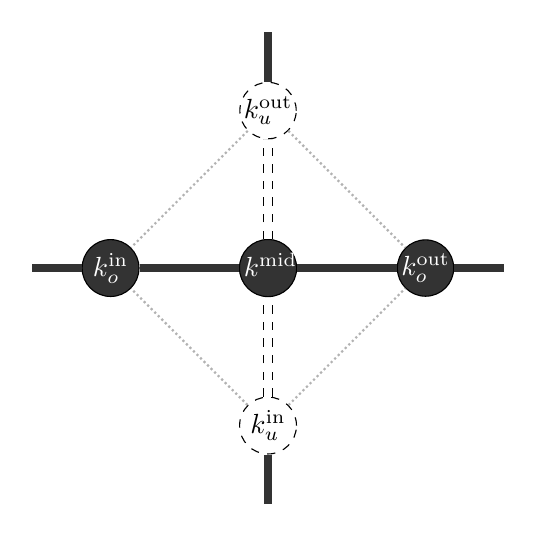
\begin{tikzpicture}[every node/.style={circle, draw, fill=none,
    inner sep=0pt, text width=1.75em, align=center}, scale=2]

  \coordinate (k)     at ( 0,  0);
  \coordinate (kuout)  at ( 0, -1);
  \coordinate (kuin) at ( 0,  1);
  \coordinate (koin)  at (-1,  0);
  \coordinate (koout) at ( 1,  0);

  \pgfmathsetmacro{\extra}{1.5}
  \coordinate (top) at (0,\extra);
  \coordinate (right) at (\extra, 0);
  \coordinate (bottom) at (0,-\extra);
  \coordinate (left) at (-\extra,0);

  % Since it's a negative crossing, we actually flip the labels from
  % what the node names are because I just repurposed the code for the
  % negative crossing case.
  \begin{scope}
    \node[dashed] (kuout) at (kuout) {$k_u^{\rm in}$};
    \node[dashed] (kuin) at (kuin) {$k_u^{\rm out}$};
  \end{scope}


  \begin{scope}
    \node[fill=black!80!white, text=white] (k) at (k) {$k_{\phantom{o}}^{\rm mid}$};
    \node[fill=black!80!white, text=white] (koin) at (koin) {$k_o^{\rm in}$};
    \node[fill=black!80!white, text=white] (koout) at (koout) {$k_o^{\rm out}$};
  \end{scope}

  \draw[line width=3pt, black!80!white] (koin) -- (k) -- (koout);
  \draw[double, double distance=3pt, dashed] (kuout) -- (k) -- (kuin);

  \draw[black!30!white, densely dotted, thick] (kuin) -- (koin) (kuout) -- (koout);
  \draw[black!30!white, densely dotted, thick] (kuin) -- (koout) (kuout) -- (koin);


  \draw[black!80!white, line width=3pt] (kuin) -- (top) (koout) -- (right) (kuout) -- (bottom)
  (koin) -- (left);

\end{tikzpicture}
\end{document}
